\documentclass[11pt,letterpaper]{article}

\usepackage[utf8]{inputenc}
\usepackage[T1]{fontenc}
\usepackage[spanish,es-nodecimaldot]{babel}
\usepackage[margin=2.5cm]{geometry}
\usepackage{amsmath,amssymb}
\usepackage{graphicx}
\usepackage{subcaption}
\usepackage{booktabs}
\usepackage{xcolor}
\usepackage{hyperref}
\usepackage{microtype}
\usepackage{fancyhdr}

\hypersetup{colorlinks=true,linkcolor=blue!70!black,urlcolor=blue!70!black}
\setlength{\headheight}{14pt}
\setlength{\emergencystretch}{2em}
\pagestyle{fancy}
\fancyhf{}
\fancyhead[L]{\small\textsl{Boletín 04: Range Queries}}
\fancyhead[R]{\small\textsl{Bryan Aguirre F. --- Mat. 2024443402}}
\fancyfoot[C]{\thepage}

\begin{document}
\hypersetup{pageanchor=false}
\begin{titlepage}
    \centering
    
\includegraphics[width=0.42\textwidth]{logo_udec.png}\\[1.0cm]
    {\scshape\Large Universidad de Concepción\par}
    \vspace{0.3cm}
    {\large Facultad de Ingeniería\par}
    {Departamento de Ingeniería Informática y Ciencias de la Computación\par}
    \vspace{2cm}
    {\Large Estructuras de Datos y Algoritmos Avanzados (2026-2)\par}
    \vspace{1cm}
    \rule{\linewidth}{0.6mm}\par
    \vspace{0.4cm}
    {\huge\bfseries Boletín 04: Range Queries\par}
    \vspace{0.4cm}
    \rule{\linewidth}{0.6mm}\par
    \vspace{1.5cm}
    \begin{minipage}[t]{0.48\textwidth}
        \raggedright
        \textbf{Autor:}\\
        Bryan Eliseo Aguirre Fuentes\\[0.3cm]
        \textbf{Matrícula:}\\
        2024443402
    \end{minipage}
    \hfill
    \begin{minipage}[t]{0.48\textwidth}
        \raggedleft
        \textbf{Profesor:}\\
        Dr. José Fuentes\\[0.3cm]
        \textbf{Ayudante:}\\
        Leonardo Lovera
    \end{minipage}
    \vfill
    {Concepción, Chile\\\today\par}
\end{titlepage}
\hypersetup{pageanchor=true}
\pagenumbering{roman}
\tableofcontents
\clearpage
\pagenumbering{arabic}

\section{Resumen}

\subsection{Propósito y alcance del estudio}

Este estudio compara dos estructuras de datos para resolver el problema de
\textit{Range Minimum Query} (RMQ): \textbf{Sparse Table} y
\textbf{Segment Tree}. Dado un arreglo de enteros \(A\), una consulta sobre
el rango inclusivo \(A[L..R]\) busca obtener el \textbf{índice del elemento
mínimo}, no solamente su valor. Se consideran un \textbf{escenario estático},
en el que el arreglo permanece fijo, y un \textbf{escenario dinámico},
en el que sus elementos reciben modificaciones puntuales.

El diseño experimental contempla cuatro comparaciones:
\begin{itemize}
    \item \textbf{Construcción en el escenario estático:} medir el tiempo
    necesario para construir ambas estructuras a partir del mismo arreglo,
    considerando diferentes cantidades de elementos.
    \item \textbf{Consultas en el escenario estático:} medir el tiempo de
    respuesta sobre las estructuras ya construidas, utilizando rangos
    aleatorios de distintas longitudes y arreglos de diferentes tamaños.
    \item \textbf{Mantenimiento en el escenario dinámico:} comparar el
    tiempo de una actualización puntual en Segment Tree con el tiempo de
    reconstruir Sparse Table después del mismo cambio. Esta comparación
    representa el costo de mantener respuestas vigentes, no dos operaciones
    de actualización equivalentes.
    \item \textbf{Consultas en el escenario dinámico:} medir el tiempo de
    respuesta después de aplicar los cambios y mantener ambas estructuras
    actualizadas, separándolo del costo de mantenimiento.
\end{itemize}

En cada comparación se utilizarán las mismas entradas y consultas para ambas
estructuras. Además, se realizará un \textbf{análisis del espacio utilizado},
considerando las asignaciones de memoria de los constructores y las reservas
temporales relevantes durante la construcción o reconstrucción. Los resultados
se interpretarán junto con las complejidades teóricas para discutir las
ventajas y limitaciones de cada alternativa. El estudio también abordará su
adaptación a otras operaciones binarias y las propiedades algebraicas que
permiten conservar sus garantías.

\subsection{Estructuras y algoritmos estudiados}

\begin{itemize}
    \item \textbf{Sparse Table:} preprocesa el arreglo almacenando resultados
    para bloques de longitud potencia de dos. Para RMQ permite responder
    consultas en tiempo constante mediante la combinación de dos bloques
    que pueden solaparse. La implementación estudiada no ofrece
    actualizaciones, por lo que en el escenario dinámico se reconstruirá
    después de cada modificación.
    \item \textbf{Segment Tree:} organiza los mínimos de intervalos en una
    estructura jerárquica. Responde consultas y permite actualizar un
    elemento en tiempo logarítmico, recalculando los nodos afectados sin
    reconstruir toda la estructura.
\end{itemize}

Las implementaciones incorporadas proceden del repositorio oficial del curso,
con autoría original de LELE \cite{edaa-sparse-table,edaa-segment-tree}.

\clearpage
\section{Análisis teórico}

Sea \(A\) un arreglo no vacío de \(n\) enteros. Una consulta RMQ sobre
\(A[L..R]\), con \(0\leq L\leq R<n\), devuelve el índice de su elemento
mínimo. Denotamos por \(k=R-L+1\) la longitud del rango y resolvemos los
empates con el \textbf{menor índice}. Para ello, cada candidato se representa
mediante el par \((A[i],i)\): el mínimo lexicográfico compara primero el valor
y luego el índice. Las implementaciones reciben intervalos semiabiertos
\([L,R+1)\); convertir los extremos y extraer el índice de la respuesta cuesta
\(\Theta(1)\).

Usamos \(O(\cdot)\) para cotas superiores y
\(\Theta(\cdot)\) para cotas ajustadas. Suponemos un modelo de palabras de
máquina: valores, índices y pares ocupan espacio constante, y acceder, copiar
y comparar un par cuesta \(\Theta(1)\). El espacio de la estructura incluye
sus copias internas, pero excluye el arreglo externo de entrada; devolver un
índice ocupa \(\Theta(1)\). Las expresiones con \(\log n\), en base dos,
se presentan para \(n\geq2\); con un solo elemento las operaciones RMQ son
constantes. El análisis se deriva del código del curso y de las descripciones
de ambas estructuras \cite{edaa-sparse-table,edaa-segment-tree,cp-sparse-table,cp-segment-tree}.

\subsection{Sparse Table}

Sparse Table almacena respuestas para bloques de longitud potencia de dos.
Si \(S_j[i]\) es el mínimo lexicográfico del bloque que comienza en \(i\)
y tiene \(2^j\) elementos, su construcción utiliza
\[
    S_0[i]=(A[i],i),\qquad
    S_j[i]=\min_{\mathrm{lex}}\bigl(S_{j-1}[i],
                              S_{j-1}[i+2^{j-1}]\bigr).
\]
La implementación reserva \(\ell=\lfloor\log_2 n\rfloor+1\) filas
completas de \(n\) elementos, aunque algunas posiciones no correspondan a
bloques válidos \cite{edaa-sparse-table}. Para una consulta, toma
\(b=\lfloor\log_2 k\rfloor\) y combina
\[
    \min_{\mathrm{lex}}\bigl(S_b[L],S_b[R-2^b+1]\bigr).
\]
Los dos bloques cubren el rango y pueden solaparse. La duplicación de su
intersección no cambia el mínimo, por la idempotencia de esta operación
\cite{cp-sparse-table}.

\begin{itemize}
    \setlength{\itemsep}{2pt}
    \setlength{\parskip}{0pt}
    \item \textbf{Preparación (construcción):} \(\Theta(n\log n)\), tanto
    en mejor como en peor caso. Inicializar las filas ya requiere
    \(\Theta(n\ell)\) trabajo. Además, si
    \(m=\lfloor\log_2 n\rfloor\), se realizan
    \(\sum_{j=1}^{m}(n-2^j+1)=m(n+1)-2^{m+1}+2\)
    combinaciones; cada una cuesta tiempo constante.
    \item \textbf{Mejor caso de consulta RMQ:} \(\Theta(1)\).
    \item \textbf{Peor caso de consulta RMQ:} \(\Theta(1)\). El método
    \texttt{query\_idempotent} realiza dos accesos y una combinación.
    Calcula el nivel con \texttt{std::bit\_width}, que permite obtener
    \(\lfloor\log_2 k\rfloor\) sobre una palabra de ancho fijo sin recorrer
    el rango \cite{cp-sparse-table,cpp-bit-width}.
    \item \textbf{Consulta general:} el método distinto \texttt{query}
    descompone \(k\) en potencias de dos y combina bloques disjuntos.
    Procesa tantos bloques como bits uno tiene \(k\): su costo es
    \(\Theta(\operatorname{popcount}(k))\), con mejor caso \(\Theta(1)\)
    y cota \(O(\log(k+1))\). No es la variante utilizada para medir RMQ.
    \item \textbf{Mantenimiento tras un cambio:} la implementación no ofrece
    \texttt{update}. En el escenario dinámico se reconstruye la tabla,
    con costo \(\Theta(n\log n)\) por modificación, independientemente
    de su posición. Es una estrategia de mantenimiento del estudio, no una
    operación de actualización nativa ni una imposibilidad de diseñar
    otras variantes.
    \item \textbf{Memoria:} \(\Theta(n\log n)\) persistente y
    \(\Theta(1)\) auxiliar por consulta. Para
    \(s=\operatorname{sizeof}(T)\), las filas contienen \(n\ell\) objetos
    de tipo \(T\), cuyo tamaño lógico de datos es \(n\ell s\) bytes,
    además de los metadatos de los vectores y del combinador. La expresión
    que crea las filas utiliza también un vector temporal de \(n\)
    elementos: \(\Theta(n)\) espacio temporal, sin cambiar el orden
    \(\Theta(n\log n)\) del pico total de construcción.
\end{itemize}

El tamaño lógico no debe confundirse con los bytes efectivamente reservados:
estos dependen de las capacidades de los vectores y de la biblioteca usada.
Si durante una reconstrucción coexisten la tabla anterior y la nueva, el pico
puede aumentar, pero conserva el mismo orden asintótico.

\subsection{Segment Tree}

Segment Tree mantiene mínimos de grupos de elementos en una jerarquía binaria
\cite{cp-segment-tree}. La versión del curso es iterativa: reserva un vector
de \(2n\) posiciones, coloca las hojas en \([n,2n)\) y calcula los nodos
internos combinando sus dos hijos. No redondea \(n\) a una potencia de dos
\cite{edaa-segment-tree}.

\begin{itemize}
    \setlength{\itemsep}{2pt}
    \setlength{\parskip}{0pt}
    \item \textbf{Preparación (construcción):} \(\Theta(n)\), tanto en mejor
    como en peor caso. Inicializa \(2n\) posiciones, copia \(n\) hojas y
    calcula exactamente \(n-1\) mínimos de hijos. No realiza \(n\)
    actualizaciones independientes, lo que costaría \(O(n\log n)\).
    \item \textbf{Mejor caso de consulta:} \(\Theta(1)\), por ejemplo al
    consultar un único elemento. En ese caso el intervalo se consume en
    una iteración del recorrido ascendente.
    \item \textbf{Peor caso de consulta:} \(\Theta(\log n)\). Los dos
    extremos ascienden dividiéndose por dos y se incorporan como máximo
    dos nodos por nivel. Existen rangos que requieren recorrer
    \(\Theta(\log n)\) niveles. Más precisamente, para longitud \(k\)
    el bucle queda acotado por \(O(\log(k+1))\), porque la cantidad de
    posiciones pendientes se reduce al menos a la mitad en cada paso.
    Por ello, mantener \(k\) fijo no obliga a observar crecimiento
    logarítmico con \(n\), aunque sí puedan variar los accesos a caché.
    \item \textbf{Actualización puntual:} \(\Theta(\log n)\) en mejor y
    peor caso para \(n\geq2\). Después de escribir una hoja, el método
    \texttt{update} recalcula todos sus ancestros hasta la raíz. No termina
    anticipadamente si el nuevo valor coincide con el anterior o si un
    mínimo intermedio no cambia.
    \item \textbf{Memoria:} \(\Theta(n)\) persistente y \(\Theta(1)\)
    auxiliar por consulta y actualización. Los \(2n\) objetos del vector
    representan \(2ns\) bytes lógicos de datos, más los metadatos y
    cualquier capacidad adicional. La construcción usa \(\Theta(1)\)
    espacio temporal fuera de ese almacenamiento, y el pico total es
    \(\Theta(n)\). Las actualizaciones no crean nuevos nodos.
\end{itemize}

Estas cotas se refieren al código iterativo incorporado, no a otra
implementación recursiva que reserve \(4n\) posiciones. En ambas estructuras,
el contenido de los valores no modifica las reservas principales ni la cantidad
de pasos de construcción; el costo de consulta del árbol depende del rango,
no de encontrar antes un valor especialmente pequeño.

\subsection{Comparación de complejidades}

La tabla resume RMQ con pares de tamaño fijo. La consulta excluye la
construcción y el mantenimiento; en Sparse Table corresponde a
\texttt{query\_idempotent}. La columna de mantenimiento compara reconstruir
Sparse Table con actualizar Segment Tree, no dos constructores.

\begingroup
\centering
\small
\begin{tabular}{@{}lccccc@{}}
\toprule
\textbf{Estructura} & \textbf{Construcción} &
\shortstack{\textbf{Mejor}\\\textbf{consulta}} &
\shortstack{\textbf{Peor}\\\textbf{consulta}} &
\textbf{Mantenimiento} & \shortstack{\textbf{Memoria}\\\textbf{persistente}} \\
\midrule
Sparse Table & \(\Theta(n\log n)\) & \(\Theta(1)\) & \(\Theta(1)\) &
\(\Theta(n\log n)\) & \(\Theta(n\log n)\) \\
Segment Tree & \(\Theta(n)\) & \(\Theta(1)\) & \(\Theta(\log n)\) &
\(\Theta(\log n)\) & \(\Theta(n)\) \\
\bottomrule
\end{tabular}
\par
\endgroup

\clearpage
\section{Implementación}

Las dos implementaciones son clases genéricas de C++20 obtenidas del
repositorio del curso y conservadas en \texttt{include/range\_queries/}.
Reciben un vector de elementos de tipo \texttt{T} y consultan intervalos
semiabiertos \([i,j)\). Para obtener el índice del mínimo se utilizaron pares
\((\text{valor},\text{índice})\), cuyo orden lexicográfico resuelve empates
por el menor índice. Se reemplazaron los comentarios y se añadió la cabecera
\texttt{<bit>} a Sparse Table, sin modificar la lógica de los algoritmos.

\subsection{Sparse Table}

La clase \texttt{sparse\_table} guarda una matriz de vectores \texttt{ST}
y una función de combinación \texttt{f}. El constructor obtiene
\(m=\lfloor\log_2 n\rfloor\) mediante \texttt{\_lg}, reserva \(m+1\)
filas de \(n\) elementos y copia la entrada en \texttt{ST[0]}. Dos ciclos
construyen las filas siguientes: \texttt{p} representa la longitud de un
bloque y \texttt{q} el doble; cada posición válida combina dos bloques
consecutivos de la fila anterior.

Para RMQ se empleó \texttt{query\_idempotent}, que calcula el nivel
\texttt{b} a partir de la longitud del intervalo y combina los bloques
de esa fila que comienzan en \(i\) y \(j-2^b\). La clase también
incluye \texttt{query}, que recorre bloques disjuntos, pero no es la variante
seleccionada para esta comparación. Como no dispone de \texttt{update},
en el escenario dinámico se reconstruyó desde el arreglo modificado.
La implementación proviene del repositorio del curso \cite{edaa-sparse-table}.

\subsection{Segment Tree}

La clase \texttt{segment\_tree} almacena la estructura en un vector
\texttt{ST} de \(2n\) elementos. El constructor copia la entrada en las
hojas, desde \texttt{ST[n]} hasta \texttt{ST[2n - 1]}, y recorre los
índices internos en orden descendente para guardar el mínimo de cada par
de hijos mediante \texttt{\_min}.

El método \texttt{query} desplaza los extremos del intervalo a las hojas e
inicializa \texttt{q} con un elemento del rango. Un ciclo asciende por el
árbol, incorpora los nodos de los bordes según la paridad de los extremos
y conserva el menor candidato. El método \texttt{update} cambia una hoja
y recalcula el mínimo de sus ancestros, combinando cada nodo con su hermano
hasta alcanzar la raíz, sin reconstruir el vector.
La implementación proviene del repositorio del curso \cite{edaa-segment-tree}.

\clearpage
\section{Metodología experimental}

\subsection{Características de la máquina}

Los experimentos se realizarán en una estación de trabajo con las siguientes
características:
\begin{itemize}
    \item \textbf{Procesador:} Intel Core i5-13420H (Raptor Lake), 8 núcleos y
    12 hilos (4 P-Cores y 4 E-Cores), frecuencia base de 2.10 GHz y turbo de
    hasta 4.60 GHz. Cachés: L1d de 320 KiB, L1i de 384 KiB, L2 de 7 MiB y L3
    compartida de 12 MiB.
    \item \textbf{Memoria principal:} 16 GiB DDR (15 GiB utilizables por el
    sistema operativo).
    \item \textbf{Almacenamiento:} SSD NVMe WD PC SN740 de 512 GB, interfaz
    PCIe Gen4 $\times$4.
    \item \textbf{Entorno de compilación:} Arch Linux x86\_64 (kernel 6.x),
    GCC y las banderas \texttt{-std=c++20 -O3 -march=native}.
    \item \textbf{Afinidad de CPU:} se fijará el proceso de medición al núcleo
    lógico 2 mediante \texttt{taskset -c 2}. Esto reduce las migraciones entre
    núcleos, pero no elimina variaciones de frecuencia, temperatura ni la
    actividad concurrente del sistema.
\end{itemize}

\subsection{Datos de entrada}

Se utilizarán \textbf{arreglos de enteros generados artificialmente}.
Para cada tamaño \(n\) se generarán tres
arreglos con valores de distribución uniforme en el intervalo
\([0,10^9]\), utilizando las semillas fijas \textbf{1729, 2718 y 31415}.
Se registrarán las semillas y los parámetros de generación para reproducir
las entradas. Sparse Table y Segment Tree recibirán exactamente los mismos
datos en cada comparación.

\begin{itemize}
    \item \textbf{Representación de los elementos:} cada entero se asociará
    con su posición mediante un par \((\text{valor},\text{índice})\).
    Ambos componentes serán enteros: el dato numérico y su posición.
    El orden lexicográfico permitirá obtener el índice del mínimo y,
    ante valores iguales, seleccionar la posición más a la izquierda.
    La preparación de estos pares quedará fuera del tiempo medido.
    \item \textbf{Consultas:} para una longitud de rango \(k\), con
    \(1\leq k\leq n\), se elegirá uniformemente una posición inicial
    \(L\) entre \(0\) y \(n-k\), y se fijará \(R=L+k-1\).
    Así, cada consulta corresponderá a un intervalo inclusivo válido
    \([L,R]\), que se traducirá a \([L,R+1)\) al invocar las
    implementaciones. Se considerarán distintas longitudes y ambas
    estructuras responderán la misma secuencia de consultas.
    \item \textbf{Actualizaciones:} en el escenario dinámico se generará
    una secuencia reproducible de posiciones elegidas uniformemente entre
    \(0\) y \(n-1\), permitiendo posiciones repetidas, y nuevos valores
    del intervalo \([0,10^9]\), distintos del valor vigente.
    Los cambios se aplicarán en el mismo orden: Segment Tree actualizará
    la hoja correspondiente y Sparse Table se reconstruirá a partir del
    arreglo modificado. El índice asociado a cada elemento se conservará.
    Las consultas posteriores serán iguales para ambas alternativas.
    \item \textbf{Entradas de validación:} se emplearán, por separado,
    arreglos pequeños crecientes, decrecientes, con todos sus elementos
    iguales, con mínimos repetidos y de un solo elemento. Estos casos
    comprobarán la corrección y el desempate; no constituirán experimentos
    temporales adicionales.
\end{itemize}

La generación de los arreglos, las consultas y la secuencia de modificaciones
se realizará antes del cronometraje. Los tamaños de arreglo, las longitudes
concretas de los rangos y las cantidades de operaciones se fijarán antes de
ejecutar los experimentos.

\subsection{Experimentos e hipótesis}

Se compararán Sparse Table y Segment Tree mediante \textbf{cuatro experimentos}:
construcción inicial y consultas en el escenario estático, y mantenimiento
y consultas posteriores a modificaciones en el escenario dinámico. Para cada
entrada se construirán ambas estructuras y se \textbf{reutilizarán las
instancias} para consultar el arreglo sin cambios. Después se aplicará la
secuencia de modificaciones: Segment Tree conservará su instancia mediante
\texttt{update}, mientras que Sparse Table será sustituida por una nueva
construcción del arreglo vigente. No se reconstruirán estructuras entre
consultas si no ha ocurrido un cambio.

El cronometraje seguirá el esquema de la plantilla \texttt{uhr}, de Leonardo
Lovera (LELE), adaptado para usar \texttt{std::chrono::steady\_clock} y
expresar los tiempos en nanosegundos \cite{lovera-uhr}. Se realizarán
\textbf{32 repeticiones por configuración y semilla}, después del
calentamiento. Las consultas estáticas se medirán en lotes calibrados fuera
de muestra, conservando el tamaño del lote entre repeticiones de una misma
configuración y método. En el escenario dinámico se respetará la carga fija
definida a continuación, sin añadir consultas para calibrar el reloj.
El tiempo de cada lote se dividirá por la cantidad de consultas ejecutadas.
La construcción y el mantenimiento se expresarán por construcción y por
modificación, respectivamente, sin mezclarlos con el tiempo de consulta.

La generación de datos, preparación de pares, validación y escritura de
resultados quedarán fuera del reloj. También se excluirá la destrucción de
las estructuras, tanto después de construir como al reemplazar Sparse Table;
en este último caso se cronometrará la creación de la tabla nueva. Los índices
devueltos se consumirán para evitar que el compilador elimine las consultas.
La corrección se contrastará con un barrido lineal independiente, fuera de
los intervalos medidos.

En cada repetición dinámica se partirá del mismo arreglo inicial y se
reproducirán los mismos cambios y consultas. La restauración del estado y el
calentamiento quedarán fuera de la muestra; dentro de la secuencia se
conservarán las instancias y su estado entre operaciones. Los experimentos
de mantenimiento y consultas dinámicas se distinguirán por sus intervalos
de cronometraje, sin duplicar una modificación en el mismo recorrido.

Se ejecutarán \textbf{10 ciclos por arreglo, semilla y repetición dinámica}.
Cada ciclo comenzará con \textbf{una actualización puntual}, seguida de
\textbf{1.000 consultas}: primero se aplicará \texttt{update} en Segment
Tree o se reconstruirá Sparse Table y, solo después, se consultará el estado
vigente. Esto supone \textbf{10 modificaciones y 10.000 consultas medidas por
estructura en cada repetición dinámica}. Las 1.000 consultas de cada ciclo
se repartirán equilibradamente entre las longitudes de rango seleccionadas,
registrando por separado el tiempo y la cantidad de consultas de cada
longitud. Así se reutilizará cada estado actualizado para todos sus lotes,
sin multiplicar las reconstrucciones al cambiar la longitud del rango.

No se forzará que las consultas aleatorias incluyan la posición modificada,
para conservar la distribución de rangos definida. Como comprobación de
corrección, después del lote se verificará también la posición actualizada
mediante una consulta unitaria fuera del cronometraje.

Se conservarán muestras crudas y resúmenes CSV con \textbf{media, desviación
estándar muestral, mínimo, Q1, mediana, Q3 y máximo}, identificando estructura,
tamaño del arreglo, longitud del rango, semilla, repetición y ciclo cuando
corresponda. Para resumir el escenario dinámico se obtendrá, en cada
repetición, el tiempo medio por modificación sobre sus diez ciclos y el
tiempo por consulta de cada longitud sobre sus lotes. Los ciclos no se
contarán como repeticiones independientes adicionales. Las figuras
mostrarán media y barras de una desviación estándar, como en el boletín
anterior; no se interpretarán como intervalos de confianza. Cada semilla
conservará su resumen: las repeticiones sobre un mismo arreglo no se tratarán
como arreglos independientes. Las diferencias se evaluarán junto con su
dispersión: las 32 repeticiones permiten caracterizar la variabilidad, pero
no garantizan por sí solas significancia estadística ni una superioridad
universal a partir de las cotas asintóticas.

Antes de la ejecución oficial se realizará un \textbf{piloto}, especialmente
con el arreglo de mayor tamaño, para estimar la duración de la matriz
completa. El presupuesto del conjunto será de \textbf{menos de una hora},
con una proyección objetivo de \textbf{45 minutos como máximo} y
\textbf{15 minutos de margen}. La estimación incluirá calentamiento,
calibración, restauración y destrucción de estructuras, validación, análisis
de memoria, escritura y generación de gráficos, aunque estas tareas estén
fuera del cronometraje de las operaciones. Si la proyección supera el
objetivo, se revisará el tamaño máximo o la cantidad de ciclos dinámicos
antes de ejecutar, manteniendo las 32 repeticiones y documentando el ajuste.
No se dará por garantizada la duración hasta comprobarla con el piloto.

\subsubsection{Construcción inicial en el escenario estático}

\begin{itemize}
    \item \textbf{Variable:} \(n\), cantidad de elementos del arreglo.
    \item \textbf{Controles:} mismos valores y pares de entrada para ambas
    estructuras, con las tres semillas definidas. Cada construcción se
    realizará desde la entrada preparada, sin incluir su generación.
    \item \textbf{Resultados:} tiempo por construcción frente a \(n\),
    mediante tablas y gráficos. Las instancias construidas se reutilizarán
    para las consultas; su costo inicial no se cargará a cada consulta.
\end{itemize}

\textbf{Hipótesis.} Se espera que Sparse Table tenga mayor tiempo de
construcción al crecer \(n\), porque prepara una tabla de tamaño
\(\Theta(n\log n)\), mientras que Segment Tree construye sus nodos en
\(\Theta(n)\). El preprocesamiento adicional de Sparse Table puede
compensarse cuando se realizan suficientes consultas estáticas, pero este
beneficio se estudiará separando ambos costos, no suponiendo que ocurre para
cualquier cantidad de consultas.

\subsubsection{Consultas en el escenario estático}

\begin{itemize}
    \item \textbf{Variables:} tamaño del arreglo \(n\) y longitud del
    rango \(k\). Se variará una manteniendo fija la otra en cada comparación.
    \item \textbf{Controles:} instancias ya construidas, sin modificaciones
    del arreglo, y mismos lotes de intervalos aleatorios. Se comparará
    \texttt{query\_idempotent} de Sparse Table con \texttt{query} de
    Segment Tree.
    \item \textbf{Resultados:} tiempo por consulta frente a \(n\) para
    longitudes fijas y frente a \(k\) para tamaños de arreglo fijos.
    La construcción inicial quedará excluida de estos tiempos.
\end{itemize}

\textbf{Hipótesis.} Se espera que Sparse Table tenga menor tiempo por
consulta al resolver RMQ con dos accesos y una combinación, de costo
\(\Theta(1)\), aprovechando su preprocesamiento. Segment Tree recorrerá
los niveles necesarios para descomponer el rango, con peor caso
\(\Theta(\log n)\). No se presupone una diferencia apreciable para todos
los rangos: los unitarios son constantes en ambas estructuras, y con \(k\)
fijo la cota del recorrido del árbol no obliga a crecer con \(n\).

\subsubsection{Mantenimiento en el escenario dinámico}

\begin{itemize}
    \item \textbf{Variable:} tamaño del arreglo \(n\), bajo modificaciones
    puntuales de sus valores.
    \item \textbf{Controles:} mismo estado inicial y misma secuencia de
    posiciones y nuevos valores. Se realizarán diez ciclos, cada uno con
    una modificación seguida de 1.000 consultas compartidas entre las
    longitudes evaluadas. Cada cambio deberá quedar reflejado antes de
    responderlas; no se agruparán modificaciones para reconstruir
    Sparse Table una sola vez.
    \item \textbf{Resultados:} tiempo por modificación frente a \(n\).
    Se medirá \texttt{update} en Segment Tree y la reconstrucción en
    Sparse Table, excluyendo las consultas y la construcción inicial.
\end{itemize}

\textbf{Hipótesis.} Se espera que Segment Tree tenga menor tiempo de
mantenimiento, ya que actualiza una hoja y sus ancestros en
\(\Theta(\log n)\), frente a reconstruir Sparse Table en
\(\Theta(n\log n)\). La diferencia debería aumentar al crecer el
arreglo. Esta comparación expresa el costo de mantener respuestas correctas
tras un cambio, no dos operaciones nativas de actualización equivalentes.

\subsubsection{Consultas en el escenario dinámico}

\begin{itemize}
    \item \textbf{Variables:} tamaño del arreglo \(n\) y longitud del
    rango \(k\), manteniendo fija una al estudiar la otra.
    \item \textbf{Controles:} mismos cambios previos y lotes de consultas.
    Antes de consultar, Segment Tree deberá estar actualizado y Sparse Table
    reconstruida, de modo que ambas representen el mismo arreglo vigente.
    Se usarán los lotes de 1.000 consultas de los diez ciclos del experimento
    de mantenimiento, sin repetir los cambios ni las reconstrucciones para
    obtener estas mediciones.
    \item \textbf{Resultados:} tiempo por consulta después de las
    modificaciones, separado del tiempo de mantenimiento registrado en el
    experimento anterior. Las respuestas deberán coincidir con el mínimo
    y el desempate definidos.
\end{itemize}

\textbf{Hipótesis.} Una vez mantenidas las estructuras, Sparse Table debería
conservar su ventaja en consultas por su costo \(\Theta(1)\); Segment Tree
mantiene su cota de peor caso \(\Theta(\log n)\). Por tanto, la ventaja
esperada de Segment Tree en un entorno con cambios se atribuye al menor costo
de mantenimiento, no necesariamente a una consulta aislada más rápida.
Los tiempos pueden diferir de los estáticos por el estado de la caché dejado
por las actualizaciones o reconstrucciones, sin que cambien estas cotas.

\subsubsection{Análisis del espacio utilizado}

Se analizarán las asignaciones de los constructores para los tamaños de
arreglo evaluados, considerando el mismo tipo de par en ambas estructuras.
Se distinguirá el almacenamiento retenido de las reservas temporales de
construcción o reconstrucción, excluyendo el arreglo externo compartido.
Cualquier seguimiento de asignaciones se realizará en una pasada separada,
sin activarlo durante el cronometraje; estos bytes no representan la memoria
residente total del proceso.

\textbf{Hipótesis.} Sparse Table requerirá más espacio al crecer \(n\),
por sus \(n(\lfloor\log_2 n\rfloor+1)\) elementos almacenados, frente
a los \(2n\) de Segment Tree. Las actualizaciones del árbol reutilizan el
vector existente, mientras que la reconstrucción de la tabla requiere nuevas
reservas y puede aumentar el pico si coexisten las versiones anterior y nueva.
Este análisis acompañará los cuatro experimentos temporales, sin constituir
un quinto experimento de tiempo.

\textit{Parámetros por concretar antes de la ejecución: tamaños de arreglos,
longitudes de rangos, cantidad de consultas estáticas y criterios de
calibración de sus lotes. Los diez ciclos dinámicos propuestos quedarán
sujetos a la validación del presupuesto mediante el piloto, sin reducir
las 32 repeticiones.}

\clearpage
\begingroup
\setlength{\intextsep}{6pt plus 2pt minus 2pt}
\setlength{\textfloatsep}{8pt plus 2pt minus 2pt}
\captionsetup{font=small,skip=4pt}
\captionsetup[subfigure]{font=small,justification=centering,skip=2pt}
\section{Resultados experimentales}

La sesión oficial \texttt{official-20261106-185540-Gmo0WTDo} completó las
32 repeticiones de cada configuración y semilla: 88.704 muestras temporales
y 72 registros de memoria. Se seleccionan cuatro gráficos de los 18 disponibles;
los restantes y los CSV se conservan en las carpetas de cada experimento.
Cada curva corresponde a una estructura y cada punto promedia, con igual
peso, las medias de las tres semillas. Las barras indican la desviación
estándar muestral entre esas tres medias, no un intervalo de confianza.
El eje horizontal es logarítmico y el vertical es lineal.

\subsection{Escenario estático: construcción y consultas}

\begin{figure}[!ht]
    \centering
    \begin{subfigure}[t]{0.49\linewidth}
        \centering
        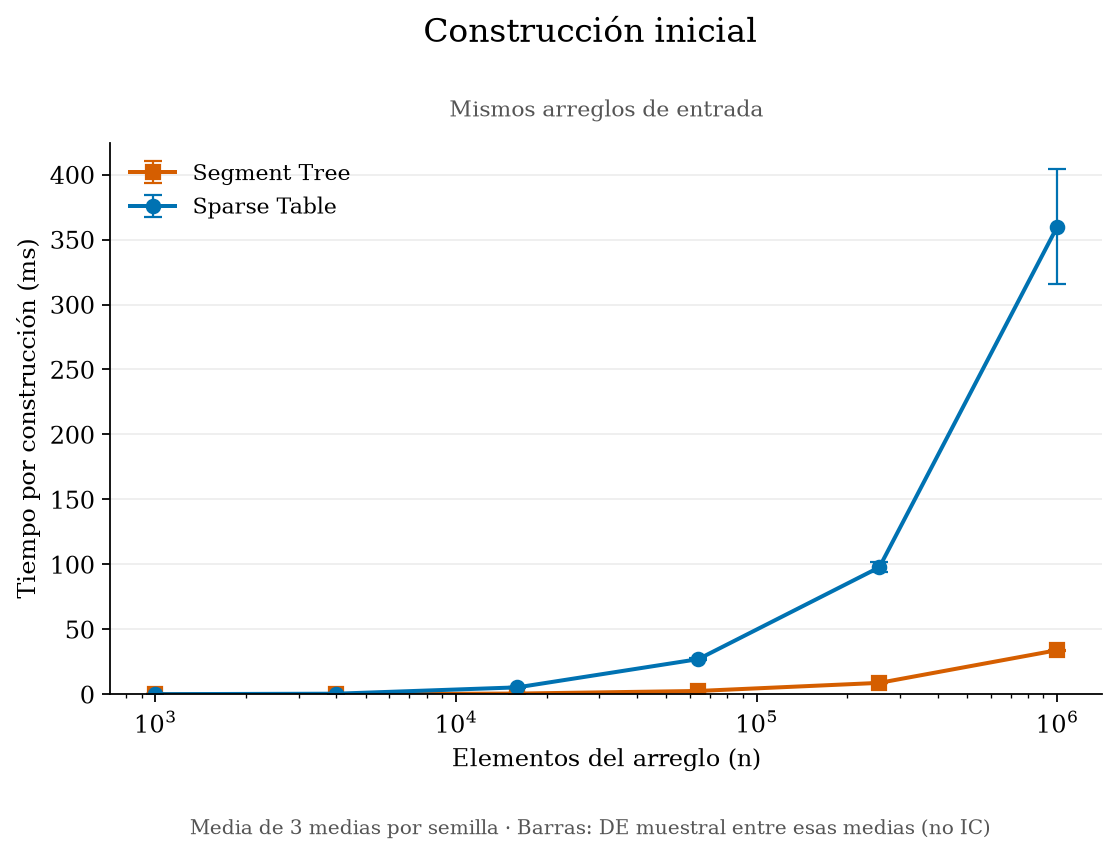
\includegraphics[width=\linewidth]{../plots/experimento_1_construccion/construction_none.png}
        \caption{Experimento 1: construcción inicial.}
        \label{fig:res-construccion}
    \end{subfigure}\hfill
    \begin{subfigure}[t]{0.49\linewidth}
        \centering
        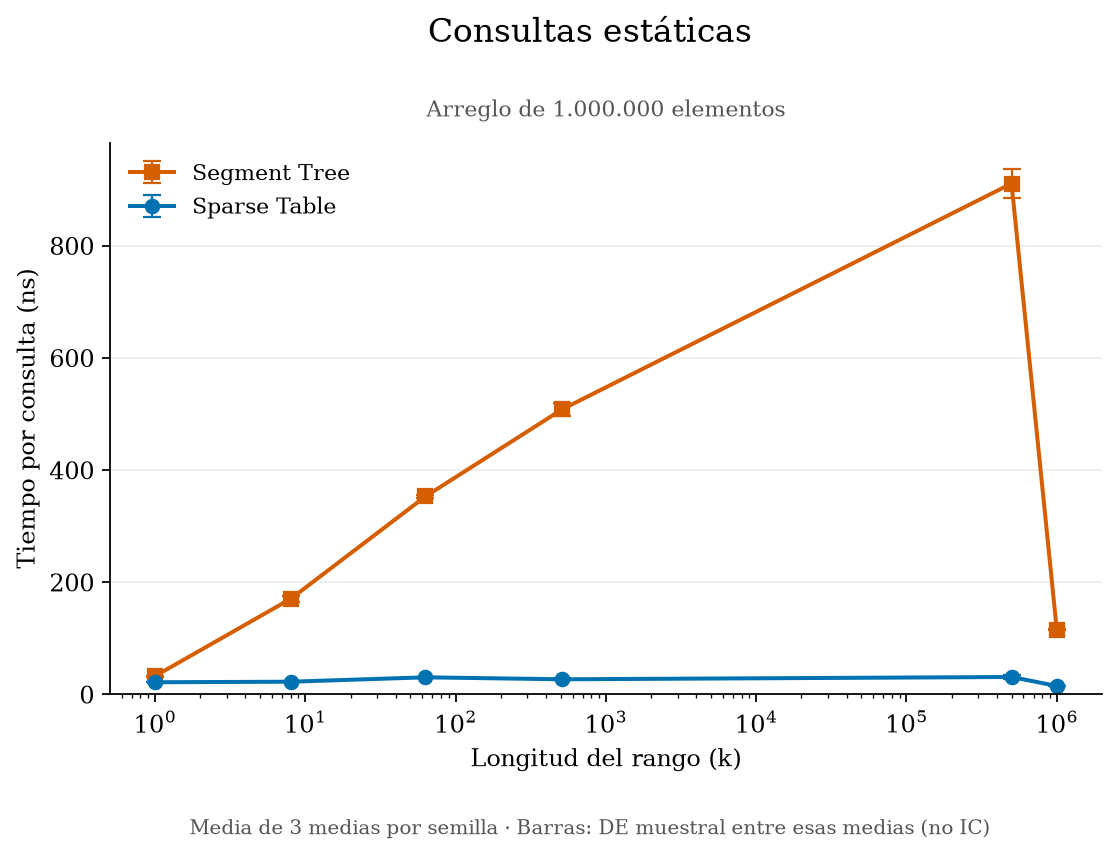
\includegraphics[width=\linewidth]{../plots/experimento_2_consultas_estaticas/static_queries_ranges_1000000.png}
        \caption{Experimento 2: consultas con \(n=10^6\).}
        \label{fig:res-consultas-estaticas}
    \end{subfigure}
    \caption{Escenario estático: costo de preparación y consultas sobre las
    estructuras ya construidas.}
    \label{fig:res-estatico}
\end{figure}

\textbf{Experimento 1.} Segment Tree presentó menor tiempo de construcción
en todos los tamaños medidos. Para \(n=10^6\), su media fue 33,953 ms,
frente a 359,880 ms de Sparse Table: una diferencia aproximada de
10,6 veces. La tendencia es consistente con las cotas \(\Theta(n)\) y
\(\Theta(n\log n)\), respectivamente, aunque estos datos no demuestran
por sí solos una complejidad asintótica.

\textbf{Experimento 2.} Sparse Table compensó parte de ese costo al consultar:
para \(n=10^6\), sus medias estuvieron entre 14,765 y 30,814 ns, frente a
32,395--910,696 ns de Segment Tree. En el rango de longitud 511, por ejemplo,
se observaron 26,714 y 507,993 ns. Este resultado se refiere a consultas
con la estructura preparada, no al costo total de una aplicación estática.
El rango completo fue más rápido que el medio en ambas estructuras;
siempre consulta el mismo intervalo \([0,n)\), por lo que no debe
interpretarse la curva como un crecimiento monótono con la longitud.

La preparación y el espacio limitan la ventaja de consultar más rápido:
con un millón de elementos, Sparse Table retuvo 305,18 MiB, frente a
30,52 MiB de Segment Tree. La tabla~\ref{tab:res-memoria} resume el espacio
sin añadir otra figura al informe.

\clearpage
\subsection{Escenario dinámico: mantenimiento y costo por ciclo}

\begin{figure}[!ht]
    \centering
    \begin{subfigure}[t]{0.49\linewidth}
        \centering
        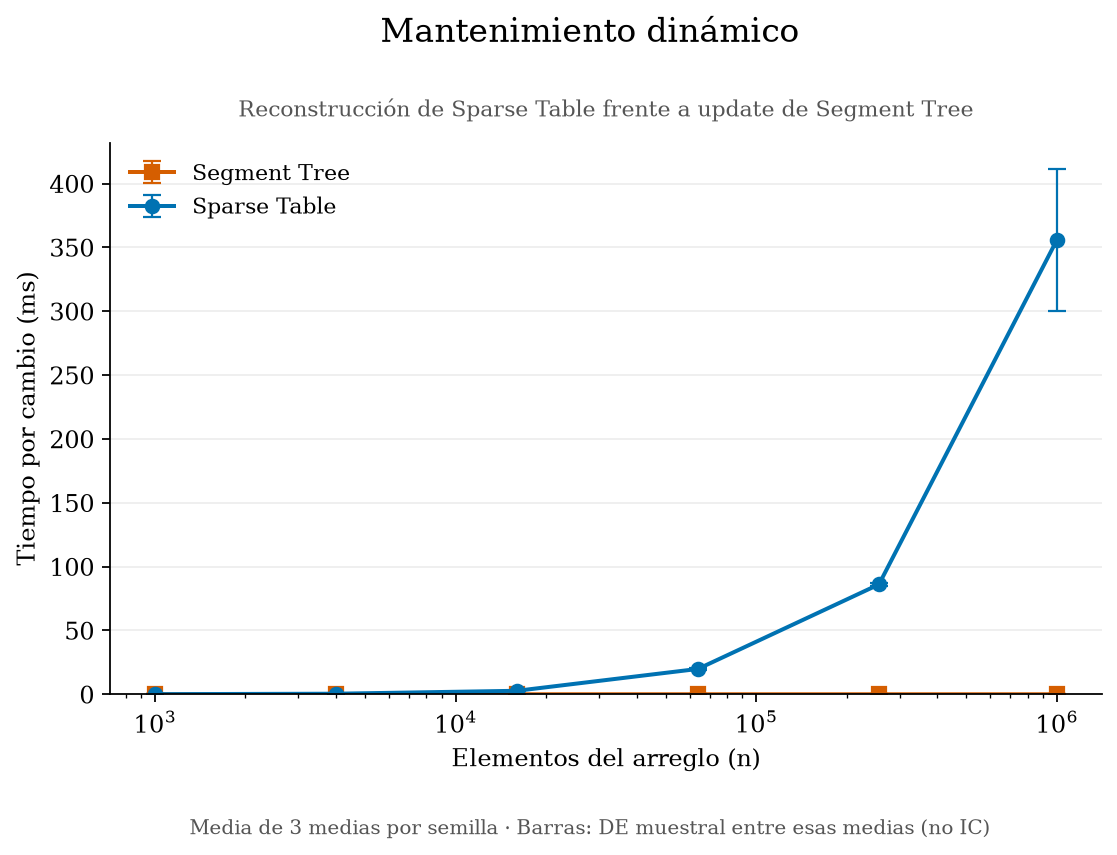
\includegraphics[width=\linewidth]{../plots/experimento_3_mantenimiento/maintenance_none.png}
        \caption{Experimento 3: reconstrucción frente a \texttt{update}.}
        \label{fig:res-mantenimiento}
    \end{subfigure}\hfill
    \begin{subfigure}[t]{0.49\linewidth}
        \centering
        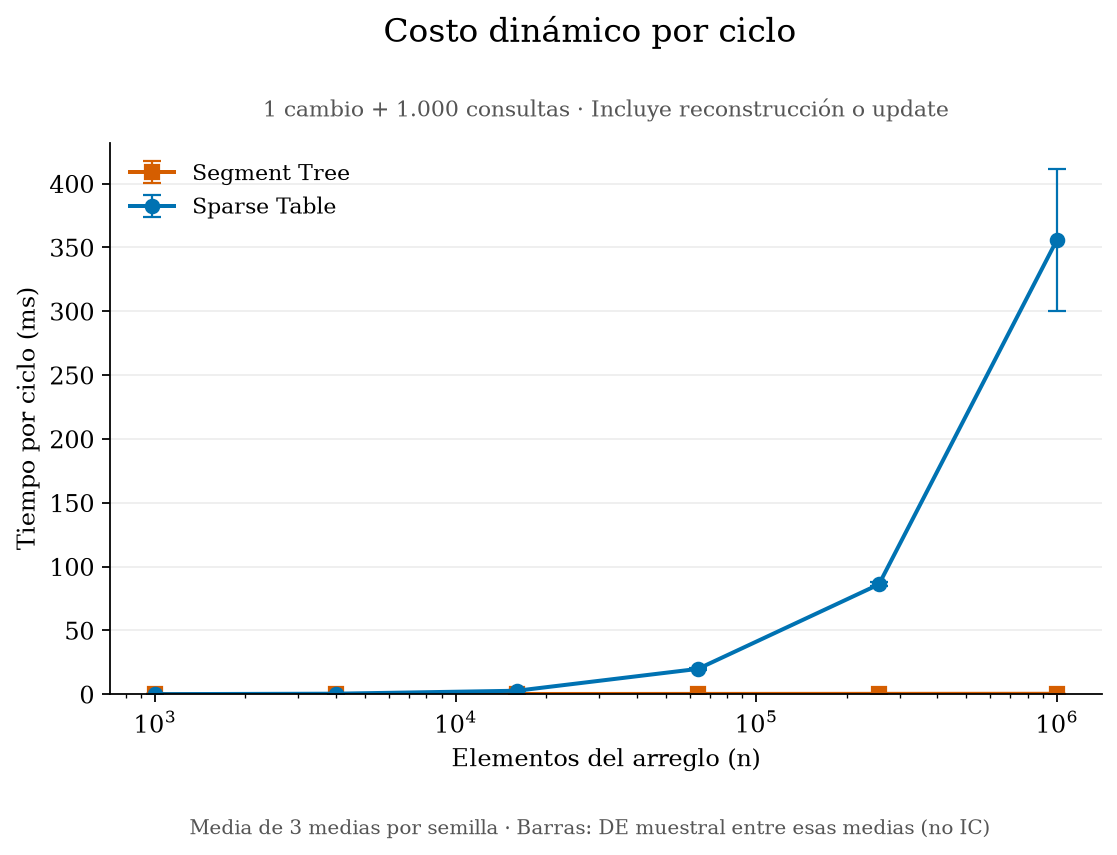
\includegraphics[width=\linewidth]{../plots/experimento_4_consultas_dinamicas/dynamic_queries_cycle.png}
        \caption{Experimento 4: un cambio y 1.000 consultas.}
        \label{fig:res-ciclo-dinamico}
    \end{subfigure}
    \caption{Escenario dinámico: mantenimiento aislado y costo combinado de
    mantenimiento y consultas del mismo ciclo.}
    \label{fig:res-dinamico}
\end{figure}

\textbf{Experimento 3.} Reconstruir Sparse Table fue más costoso que actualizar
Segment Tree en todos los tamaños. Para \(n=10^6\), las medias fueron
355,673 ms por reconstrucción y 0,831~\(\mu\)s por \texttt{update}.
Las unidades distintas de la tabla~\ref{tab:res-mantenimiento} evitan
redondear a cero las actualizaciones del árbol. Su curva casi coincide
con el eje horizontal en la figura por la diferencia de escalas,
no porque el mantenimiento sea gratuito.

\textbf{Experimento 4.} Al incluir el cambio y las 1.000 consultas de cada
ciclo, Sparse Table fue más rápida únicamente con 1.000 elementos:
0,105 ms frente a 0,156 ms. Segment Tree obtuvo menor tiempo desde
4.000 elementos entre los tamaños probados. Para \(n=10^6\), los costos
fueron 355,736 y 0,387 ms, respectivamente, unas 919 veces a favor del árbol.
El cambio de ganador se encuentra entre 1.000 y 4.000 elementos para
esta carga; no se determinó su posición exacta ni se generaliza a otra
proporción de modificaciones y consultas.

El costo por ciclo suma los intervalos de mantenimiento y consultas del
mismo método, tamaño, semilla, repetición y ciclo. La reconstrucción se
cuenta una sola vez, no por longitud de rango. Se excluyen la construcción
inicial, generación, validación, escritura y liberación: es una suma de
componentes medidos, no un cronómetro continuo de extremo a extremo.
Los diez ciclos se promedian dentro de cada repetición antes de obtener
la media por semilla; no constituyen diez repeticiones independientes.

En conjunto, las mediciones favorecen Sparse Table para consultar datos
estáticos y Segment Tree para esta carga dinámica sobre arreglos grandes.
La desviación entre semillas describe diferencias de entrada y condiciones
de ejecución que el diseño no permite separar causalmente; no se presenta
como prueba de significancia estadística.

\clearpage
% Fuentes plot_summary csv y memory_plot_summary csv de cada experimento
% Redondeo posterior a la conversion de unidades
\subsection{Resumen numérico de tiempos y memoria}

Se presentan cuatro tablas con todos los tamaños medidos. Construcción y
mantenimiento comparten las filas de \(n\), sin mezclar sus mediciones.
Los tiempos se expresan como media \(\pm\) desviación estándar muestral
entre las tres medias por semilla, con igual peso. Cada media por semilla
procede de 32 repeticiones: no es la desviación de 96 ejecuciones agrupadas
ni un intervalo de confianza. La variación dentro de cada semilla se
conserva en \texttt{summary.csv}.

\begingroup
\small
\setlength{\tabcolsep}{7pt}
\renewcommand{\arraystretch}{1.25}

\begin{table}[!ht]
    \centering
    \caption{Experimentos 1 y 3: construcción inicial y mantenimiento por cambio.}
    \label{tab:res-construccion}
    \label{tab:res-mantenimiento}
    \begin{tabular}{@{}rcccc@{}}
        \toprule
        & \multicolumn{2}{c}{Construcción inicial} & \multicolumn{2}{c}{Mantenimiento} \\
        \cmidrule(lr){2-3}\cmidrule(l){4-5}
        Elementos & Sparse Table & Segment Tree & Sparse Table & Segment Tree \\
        \(n\) & [ms] & [ms] & [ms] & [\(\mu\)s] \\
        \midrule
        1.000 & \(0{,}090 \pm 0{,}003\) & \(0{,}025 \pm 0{,}001\) & \(0{,}087 \pm 0{,}003\) & \(0{,}340 \pm 0{,}015\) \\
        4.000 & \(0{,}444 \pm 0{,}042\) & \(0{,}095 \pm 0{,}010\) & \(0{,}437 \pm 0{,}047\) & \(0{,}384 \pm 0{,}039\) \\
        16.000 & \(5{,}317 \pm 0{,}356\) & \(0{,}550 \pm 0{,}047\) & \(2{,}733 \pm 0{,}221\) & \(0{,}446 \pm 0{,}041\) \\
        64.000 & \(27{,}058 \pm 1{,}060\) & \(2{,}551 \pm 0{,}156\) & \(19{,}841 \pm 0{,}862\) & \(0{,}596 \pm 0{,}005\) \\
        256.000 & \(97{,}741 \pm 3{,}915\) & \(8{,}775 \pm 0{,}011\) & \(86{,}037 \pm 1{,}489\) & \(0{,}716 \pm 0{,}010\) \\
        1.000.000 & \(359{,}880 \pm 44{,}177\) & \(33{,}953 \pm 0{,}419\) & \(355{,}673 \pm 55{,}479\) & \(0{,}831 \pm 0{,}026\) \\
        \bottomrule
    \end{tabular}
    \par\smallskip
    \begin{minipage}{\linewidth}
        \footnotesize
        El mantenimiento compara reconstruir Sparse Table con \texttt{update}
        de Segment Tree. Solo esta última columna está en microsegundos.
    \end{minipage}
\end{table}

\begin{table}[!ht]
    \centering
    \caption{Experimento 2: tiempo por consulta estática con \(n=10^6\).}
    \label{tab:res-consultas-estaticas}
    \begin{tabular}{@{}rcc@{}}
        \toprule
        Rango & Sparse Table & Segment Tree \\
        \(k\) & [ns] & [ns] \\
        \midrule
        1 & \(21{,}436 \pm 0{,}199\) & \(32{,}395 \pm 0{,}938\) \\
        8 & \(22{,}387 \pm 0{,}752\) & \(170{,}172 \pm 5{,}207\) \\
        63 & \(30{,}239 \pm 1{,}315\) & \(352{,}761 \pm 2{,}321\) \\
        511 & \(26{,}714 \pm 1{,}720\) & \(507{,}993 \pm 11{,}615\) \\
        500.000 & \(30{,}814 \pm 3{,}387\) & \(910{,}696 \pm 26{,}032\) \\
        1.000.000 & \(14{,}765 \pm 0{,}336\) & \(114{,}839 \pm 1{,}023\) \\
        \bottomrule
    \end{tabular}
\end{table}

\begin{table}[!ht]
    \centering
    \caption{Experimento 4: tiempo por ciclo de un cambio y 1.000 consultas.}
    \label{tab:res-ciclo-dinamico}
    \begin{tabular}{@{}rcc@{}}
        \toprule
        Elementos & Sparse Table & Segment Tree \\
        \(n\) & [ms] & [ms] \\
        \midrule
        1.000 & \(0{,}105 \pm 0{,}004\) & \(0{,}156 \pm 0{,}003\) \\
        4.000 & \(0{,}457 \pm 0{,}049\) & \(0{,}182 \pm 0{,}018\) \\
        16.000 & \(2{,}772 \pm 0{,}222\) & \(0{,}218 \pm 0{,}015\) \\
        64.000 & \(19{,}889 \pm 0{,}864\) & \(0{,}284 \pm 0{,}005\) \\
        256.000 & \(86{,}090 \pm 1{,}488\) & \(0{,}332 \pm 0{,}007\) \\
        1.000.000 & \(355{,}736 \pm 55{,}485\) & \(0{,}387 \pm 0{,}003\) \\
        \bottomrule
    \end{tabular}
\end{table}

\begin{table}[!ht]
    \centering
    \caption{Memoria retenida y pico total durante el mantenimiento.}
    \label{tab:res-memoria}
    \begin{tabular}{@{}rrrrr@{}}
        \toprule
        & \multicolumn{2}{c}{Sparse Table} & \multicolumn{2}{c}{Segment Tree} \\
        \cmidrule(lr){2-3}\cmidrule(l){4-5}
        Elementos & Retenida & Pico total & Retenida & Pico total \\
        \(n\) & [MiB] & [MiB] & [MiB] & [MiB] \\
        \midrule
        1.000 & 0{,}15 & 0{,}32 & 0{,}03 & 0{,}03 \\
        4.000 & 0{,}73 & 1{,}53 & 0{,}12 & 0{,}12 \\
        16.000 & 3{,}42 & 7{,}08 & 0{,}49 & 0{,}49 \\
        64.000 & 15{,}63 & 32{,}23 & 1{,}95 & 1{,}95 \\
        256.000 & 70{,}31 & 144{,}53 & 7{,}81 & 7{,}81 \\
        1.000.000 & 305{,}18 & 625{,}61 & 30{,}52 & 30{,}52 \\
        \bottomrule
    \end{tabular}
\end{table}

\endgroup

\endgroup

\clearpage
\section{\textquestiondown Qué opción utilizar?}

\textbf{Construcción y consultas estáticas.} Los resultados respaldan las
dos primeras hipótesis: Segment Tree se construyó más rápido en todos los
tamaños, mientras que Sparse Table presentó menores tiempos por consulta
en las seis longitudes evaluadas con \(n=10^6\). Para ese tamaño, construir
costó 33,953 ms y 359,880 ms, respectivamente
(tabla~\ref{tab:res-construccion}); en rangos de longitud 511, consultar
costó 507,993 ns y 26,714 ns (tabla~\ref{tab:res-consultas-estaticas}).
Esto es consistente con la preparación \(\Theta(n)\) del árbol frente a
\(\Theta(n\log n)\) de la tabla, y con las consultas RMQ \(\Theta(1)\)
de esta última. No implica que toda consulta del árbol cueste
\(\Theta(\log n)\): los rangos unitarios son constantes en ambas
estructuras. Tampoco demuestra que la tabla amortice su preparación con
cualquier cantidad de consultas.

\textbf{Mantenimiento y carga dinámica.} La tercera hipótesis también
queda respaldada: actualizar Segment Tree fue más barato que reconstruir
Sparse Table en todos los tamaños. Con \(n=10^6\), los tiempos fueron
0,831~\(\mu\)s y 355,673 ms por cambio
(tabla~\ref{tab:res-mantenimiento}). La cuarta hipótesis se cumple para
la carga estudiada: con un cambio y 1.000 consultas por ciclo, el árbol
ganó desde 4.000 elementos; con un millón, necesitó 0,387 ms frente a
355,736 ms. Sin embargo, Sparse Table ganó con 1.000 elementos
(0,105 ms frente a 0,156 ms), por lo que no existe un ganador universal
(tabla~\ref{tab:res-ciclo-dinamico}). El cruce observado entre 1.000 y
4.000 elementos no determina un umbral exacto ni se extrapola a otras cargas.

\textbf{Espacio utilizado.} La quinta hipótesis queda respaldada por
las reservas medidas: con un millón de elementos, Sparse Table retuvo
305,18 MiB frente a 30,52 MiB del árbol, unas diez veces más. Además,
su pico al reconstruir alcanzó 625,61 MiB por la coexistencia de versiones
y reservas temporales; Segment Tree mantuvo 30,52 MiB al actualizar
(tabla~\ref{tab:res-memoria}). Son asignaciones de las estructuras,
no la memoria residente total del proceso.

\textbf{Ventajas y desventajas.} La principal ventaja de Sparse Table
es responder RMQ en tiempo constante y con menores tiempos observados
por consulta; sus desventajas son la preparación y el espacio
\(\Theta(n\log n)\), junto con la ausencia de actualización nativa en
la implementación evaluada, que obliga a reconstruir en este estudio.
Segment Tree ofrece construcción y espacio \(\Theta(n)\), además de
actualizaciones puntuales \(\Theta(\log n)\) sin nuevas reservas.
Su desventaja es un mayor costo de consulta, con peor caso
\(\Theta(\log n)\), que puede acumularse en cargas intensivas de lectura.

\textbf{En resumen.} Conviene Sparse Table para datos inmutables y
memoria suficiente, cuando el ahorro en muchas consultas amortice su preparación.
Conviene Segment Tree si hay cambios frecuentes, memoria limitada o pocas
consultas que no compensen construir la tabla. La decisión debe considerar
construcción, mantenimiento y consultas en conjunto, no solo la operación
más rápida de cada estructura. Estas conclusiones describen las mediciones
y son compatibles con las hipótesis teóricas; no constituyen una prueba
de complejidad asintótica ni de significancia estadística.

\clearpage
\begin{thebibliography}{9}
\raggedright
\phantomsection
\addcontentsline{toc}{section}{Referencias}

\bibitem{edaa-sparse-table}
LELE. \textit{Generic Sparse Table} [Código fuente].
Repositorio del curso EDAA.
\url{https://github.com/jfuentess/edaa/blob/550e2199f82e74e38d253eba2e64f8c72af38296/rmq/sparse_table.cpp}.

\bibitem{edaa-segment-tree}
LELE. \textit{Generic Segment Tree for RMQs} [Código fuente].
Repositorio del curso EDAA.
\url{https://github.com/jfuentess/edaa/blob/550e2199f82e74e38d253eba2e64f8c72af38296/rmq/segment_tree.cpp}.

\bibitem{cp-sparse-table}
Colaboradores de CP-Algorithms.
\textit{Sparse Table}.
\url{https://cp-algorithms.com/data_structures/sparse-table.html}.

\bibitem{cp-segment-tree}
Colaboradores de CP-Algorithms.
\textit{Segment Tree}.
\url{https://cp-algorithms.com/data_structures/segment_tree.html}.

\bibitem{atcoder-segtree}
AtCoder Library.
\textit{Segtree}: documentación de árboles de segmentos sobre monoides.
\url{https://atcoder.github.io/ac-library/production/document_en/segtree.html}.

\bibitem{cpp-bit-width}
Cppreference.
\textit{std::bit\_width}.
\url{https://en.cppreference.com/w/cpp/numeric/bit_width.html}.

\bibitem{cp-euclid}
Colaboradores de CP-Algorithms.
\textit{Euclidean algorithm for computing the greatest common divisor}.
\url{https://cp-algorithms.com/algebra/euclid-algorithm.html}.

\bibitem{cpp-lcm}
Cppreference.
\textit{std::lcm}.
\url{https://en.cppreference.com/w/cpp/numeric/lcm.html}.

\bibitem{lovera-uhr}
Lovera, L. (LELE). (s.\,f.).
\textit{uhr: generic time performance tester} [Código fuente].
Plantilla de medición de la ayudantía, disponible en
\texttt{utils/uhr.cpp} del repositorio de estos boletines.
Referencia del autor utilizada en los boletines anteriores:
\url{https://github.com/leonardlover}.

\par\medskip
\noindent\textbf{Declaración de uso de IA generativa.}
Se utilizaron herramientas de inteligencia artificial generativa como apoyo para las implementaciones de los experimentos y para revisar la redacción técnica de este informe. Codex se utilizó como agente prioritario durante este proceso. El autor es responsable de las decisiones finales, la verificación de los resultados y el contenido presentado.

\end{thebibliography}


\end{document}
